% Mecánico rotacional: inercia J con torque T y fricción B en el cojinete
\documentclass[border=5pt]{standalone}
\usepackage{tikz}
\usetikzlibrary{arrows.meta, patterns}
\begin{document}
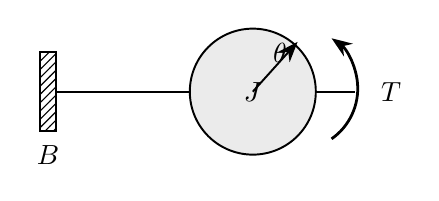
\begin{tikzpicture}[>={Stealth[length=2.6mm]}, line width=0.7pt]
  % cojinete (con friccion B)
  \fill[pattern=north east lines] (-2.7,-0.5) rectangle (-2.5,0.5);
  \draw (-2.7,-0.5) rectangle (-2.5,0.5);
  \node[below] at (-2.6,-0.55) {$B$};
  % eje
  \draw (-2.5,0) -- (-0.8,0);
  % disco (inercia J)
  \draw[fill=black!8] (0,0) circle (0.8);
  \node at (0,0) {$J$};
  \draw (0.8,0) -- (1.3,0);
  % angulo theta
  \draw[->] (0,0) -- (48:0.85);
  \node at (55:0.6) {$\theta$};
  % torque aplicado (flecha curva)
  \draw[->, line width=1pt] (1.0,-0.6) arc (-55:55:0.78);
  \node[right] at (1.5,0.0) {$T$};
\end{tikzpicture}
\end{document}
